\documentclass[11pt]{article}

\usepackage{graphicx}

% Enable references to labels in the notes
\usepackage{xr-hyper}
\externaldocument{p328_notes}
\usepackage{hyperref}

% Sans fonts
\usepackage{sfmath}
\renewcommand{\familydefault}{\sfdefault}

\newcommand{\COURSE}{PHYS328W}
\newcommand{\LABNUM}{5}
\newcommand{\TITLE}{Diode Circuits}
\markright{\COURSE~Lab \LABNUM\ : \TITLE}

\setlength{\textwidth} {6.5 true in}
\setlength{\textheight}{9 true in}
\setlength{\hoffset}   {-0.75 true in}
\setlength{\voffset}   {-0.75 true in}
\setlength{\parindent} {12 pt}
\pagestyle{myheadings}

\begin{document}

\thispagestyle{empty}

\section*{\COURSE\ Lab \LABNUM\ : \TITLE}

This assignment relies on Section~\ref{sec:diodes} of the notes.

\subsection*{Experiments}

\subsubsection*{Diode - Resistor Voltage Divider}

\begin{figure}[h]
\centering
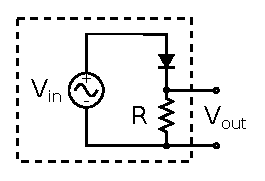
\includegraphics{diodevdivider.eps}
\caption{A diode - resistor voltage divider}
\label{fig:diodevdivider}
\end{figure}
The circuit in Figure~\ref{fig:diodevdivider} is called a
\textbf{half-wave recitfier}.  Investigate both the \texttt{1N4148}
and \texttt{1N5711} diodes as follows.

\begin{enumerate}
\item Construct the circuit in Figure~\ref{fig:diodevdivider} using a
  10~k$\Omega$ resistor.
  
\item Display $V_{in}$ and $V_{out}$ together on the oscilloscope. Use
  the cursors to measure the difference in peak voltage of these
  signals. Make sure you do not include a arbitrary DC offset between
  channels. This difference is the forward voltage drop of the diode.
\end{enumerate}

\subsubsection*{Full-Wave Bridge Rectifier}

\begin{figure}[h]
\centering
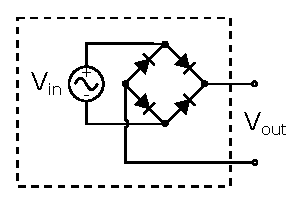
\includegraphics{bridgerectifier.eps}
\caption{A full-wave bridge rectifier.}
\label{fig:bridgerectifier}
\end{figure}
The arrangement of four diodes in Figure~\ref{fig:bridgerectifier} is
called a \textbf{full-wave bridge rectifier}. It is a key component
used in the conversion of AC to DC power in power supplies and
automotive charging systems. 

\begin{enumerate}
\item Construct the circuit in
  Figure~\ref{fig:bridgerectifier} using four \texttt{1N4148} diodes
  and a 10~k$\Omega$ load resistor.

\item Use the function generator as your AC voltage source. Drive the
  circuit at 1~kHz. 
  
\item Display $V_{in}$ and $V_{out}$ together on the oscilloscope.

\item Measure the amplitude of the input signal $|V_{in}|$ the peak
  voltage of the output signal $V_{out}$.
\end{enumerate}

\subsection*{Simulation}

\begin{enumerate}
\item Construct the full-wave bridge rectifier shown in
  Figure~\ref{fig:bridgerectifier} using standard PSpice diodes
  and a 10~k$\Omega$ load resistor.

\item Set up a transient analysis over a couple of periods of the
  input signal, and set the maximum step size so that 100
  points are plotted per period.

\item As you did for the actual circuit, measure the amplitude of the
  input signal $|V_{in}|$ and the peak voltage of the output signal of
  the bridge rectifier $|V_{out}|$.
  
\end{enumerate}

\subsection*{Products}

Upload to Canvas a brief \LaTeX\ report in which you ...
\begin{itemize}
\item Report the forward voltage drop measurements of the
  \texttt{1N4148} and \texttt{1N5711} diodes.

\item Include as a figures simulated plots of $V_{in}$
  and $V_{out}$ vs. time for the full-wave bridge rectifier.

\item Comment on ...
  \begin{itemize}
    \item any discrepancies between measurements and
      simulations.

  \item the impact of the forward diode drop on the behavior
    of the full-wave bridge rectifier.
  \end{itemize}

\end{itemize}

\end{document}
